\documentclass[12pt,titlepage]{article}

\usepackage[ngerman]{babel}
\usepackage[utf8]{inputenc}
\usepackage{color, colortbl}
\usepackage[table,xcdraw]{xcolor}
\usepackage{graphicx}
\usepackage{float}
\restylefloat{table}
\usepackage{amssymb}
\usepackage{varioref}
\usepackage[left=3cm,
  right=2cm,
  top=2.5cm,
  bottom=2cm,
  ]{geometry}

\def\code#1{\texttt{#1}}


\begin{document}

\section*{Weitere Designkonzepte im Fallbeispiel} 
Der Elektronikhersteller Regularsoft hat eine neue Taskforce gegründet, zur Analyse von alternativen Produktdesigns für sein Produktportfolio, bestehende aus Smartphones, Tablet, Notebooks und anderen technischen Geräten für den digitalen Arbeitsplatz. Grundlage für diese Entscheidung ist der globale Anstieg im Verbrauch von Kupfer und anderen Rohstoffen, welche essenziell für die einzelnen Komponente des Produktportfolios sind. Daneben wird auch innerhalb großer Teile der Kundengruppe von Regularsoft die Forderung nach umweltfreundlichen Produkten stärker. Mittlerweile nutzen einige Kunden kostengünstigere und umweltfreundlichere Alternativen der Konkurrenz. Vor allem im Bereich Smartphones und Notebook.
Mit den Ergebnissen der Taskforce will der Elektronikhersteller die ersten strategischen Schritte setzen, um seine Langzeitziel eines CO2-neutralen Unternehmens zu erreichen.


\paragraph{\textbf{BETRIEBLICHE KENNZAHLEN $\triangleright$}}
Für die Strategiefindung der Taskforce stellen die betrieblichen Kennzahlen der Regularsoft GmbH wichtige Grundsätze. Das Unternehmen konnte das letzte Geschäftsjahr mit folgenden Kennzahlen am 31.12.2020 abschließen:
\begin{itemize}
\item[•] Bilanzsumme (Mio. GE):		721,80
\item[•] Kapital (Mio. GE):			153,10
\item[•] Gesamtumsatz (Mio. GE):	980,40
\item[•] Jahresüberschuss (Mio. GE):	216,67
\end{itemize}
Für das angebrochen Geschäftsjahr hat der Finanzausschuss ein Jahreskapital von 14,6  Mio. GE für die Abteilung Marketing freigegeben. Außerdem wurden im Bereich Forschung \& Entwicklung 600 neue Mitarbeiter eingestellt und 80 weitere für die Vertriebsgruppen des Unternehmens.

\paragraph{\textbf{SONSTIGE KENNZAHLEN $\triangleright$}}
Im Rahmen der jährlicher interner und externer Untersuchungen haben sich des Weiteren folgende Ergebnisse zur Marktposition der Regularsoft ergeben:
\begin{itemize}
\item[•] \textbf{Nachfrage der Geräte:}
Umfragen bei Kunden ergaben, dass 91\% aller Neukunden auch für weitere Technikanschaffungen sich für Regularsoft-Produkte entscheiden würden. Bei Bestandskunden liegt diese Zahl sogar bei 95\%. Darüber hinaus gaben annähernd 75\% aller Geschäftskunden, so wie 81\% aller Privatkunden an, dass sie mit der Qualität der Produkte zufrieden sind und Regularsoft als Hersteller weiterempfehlen würden. Bereits in der Vergangenheit zeigte sich, dass die Nachfrage selbst bei kontroversen Produktneuerungen nur minimale fiel, aber im weiteren Zeitverlauf sich stabilisierte oder wieder anstieg.
\item[•] \textbf{Nachfrage des Betriebssystem:}
Das Betriebssystem von Regularsoft für Smartphones, Century-OS, belegt mit einem Marktanteil von 15,7\% den dritten Platz im globalen Markt. Dabei verwenden sowohl Firmen als auch privat Personen Century-OS als Betriebssystem für die betrieblichen, bzw. privaten Mobilgeräte. Innerhalb von Deutschland besitzt laut Marktforschungen jeder fünfte Haushalt ein mobiles Endgerät mit dem Century-OS.
\end{itemize}

\paragraph{\textbf{L"OSUNGANS"ATZE $\triangleright$}}
Während der Untersuchung haben sich zwei konkrete Konzepte für umweltfreundliche Produktdesigns hervorgehoben. 
\begin{itemize}
\item[•] \textbf{Modulares Produktdesign:}
Modularität im Design von Produkten definiert den Aufbau eines Produktes so, dass jede Komponente auf struktureller Sichtweise selbstständig sind und nur über bestimmte Schnittstellen verbunden sind. Dadurch wird eine dauerhafte Verbindung unter den Komponenten vermieden. Dies ermöglicht es einzelne Bestandteile einfacher aus einem Gerät zu entfernen und somit auszutauschen oder zu reparieren. Für die Nutzer der Geräte öffnet dies auch die Möglichkeit selbständig Komponenten eines Geräts auszutauschen, ohne dabei zu Techniker oder Partnerunternehmen der Hersteller gehen zu müssen. Jedoch setzt diese Funktion in manchen Fällen technische Grundkenntnisse und eine kleine Ausstattung an Werkzeug zur die Lösung der Befestigungen voraus. Wobei es dabei lediglich um Standardwerkzeug wie z.B. Schraubenziehern handelt. Im Smartphone und Tablet Bereich haben bereits mehrere Kleinunternehmen innerhalb den letzten Jahren Geräte mit modularen Design an den Markt gebracht. Für die Hersteller solcher Produkte bietet sich durch die offenen Architektur der Produkte die Möglichkeit periodisch neuer Hardwarekomponenten zu entwickeln und den Kunden als Upgrade-Varianten anzubieten. Somit lässt sich die Nutzungsdauer erhöhen, ohne dass die Geräte schnell technisch veralten und senkt durch die massenhafte Produktion von neueren Modellen die Umweltbelastung eines Unternehmens. Des Weiteren können die wertvollen Rohstoffe alter und nicht mehr genutzter Komponenten leicht recycelt werden.\\
\item[•] \textbf{Langlebige Software:}
Der Begriff "langlebige Software" beschreibt Betriebssysteme bzw. Anwendungen, welche durch spezielle, modulare Architekturen und erweiterten Support eine überdurchschnittliche Nutzungsdauer aufweisen können. Ziel dieser langlebigen Software ist es, auch ältere Geräte mit teilweise schwacher Hardware weiterhin unterstützen zu können und dadurch auch die Gesamtnutzungsdauer des Produktes zu verlängern. Erreicht wird die verlängerte Nutzungsdauer durch eine Maximierung der Kompatibilität bezüglich der Hardware, aber auch durch Transparenz gegenüber dem Benutzer. D.h. es wird genau kommuniziert, welche Änderungen ein Update zu Folge hat und der User kann frei entscheiden, ob er dieses durchführen oder ggf. auf eine ältere Softwareversion zurückkehren will. Die verwendeten modularen Architekturen ermöglichen dabei eine einfache Anpassung der Software an die Leistung der vorliegenden Hardware. Neue, ressourcenintensive Funktionen können auf diese Weise bei der Installation ausgelassen werden, während das Endgerät dennoch mit den aktuellen Sicherheits- und Kompatibilitätsupdates versorgt werden kann. Da in der Regel ein Ungleichgewicht zwischen potentieller Nutzungsdauer der Hardware und Nutzungsdauer der Software besteht, ist es mit dem Einsatz langlebiger Software möglich das Verhältnis der beiden Aspekte zu optimieren und somit sozusagen einen besseren Wirkungsgrad der Produkte zu erzielen.\\
Profitieren von dieser Praktik tut einerseits der Endkunde, da das Gerät in längeren Abständen ersetzt werden muss, was den Kunden wiederum dazu bewegen kann mehr Geld zu investieren, auf der anderen Seite profitiert auch die Natur, da längere Nutzungszyklen gleichzeitig weniger Elektroschrott bedeuten. 
\end{itemize}


\paragraph{\textbf{SWOT-ANALYSE DER LÖSUNGSANSÄTZE  $\triangleright$}}
Nach Untersuchung beider Lösungs- ansätze hat die Regularsoft entschieden beide Varianten zu nutzen und sie als Basis für die nächsten Generationen des Produktportfolios anzuwenden. Somit kann Regularsoft sich lange Zeit für die Entwicklung der darauffolgenden Generationen konzentrieren und die Nachfrage durch modulare Upgrades beibehalten. Mit den Neuerungen kann das Unternehmen auch einige Materialien in den alten Komponenten recyceln. Grundlage für diese Entscheidung war folgende SWOT-Analyse der Taskforce:\\

\begin{figure}[h]
 \centering
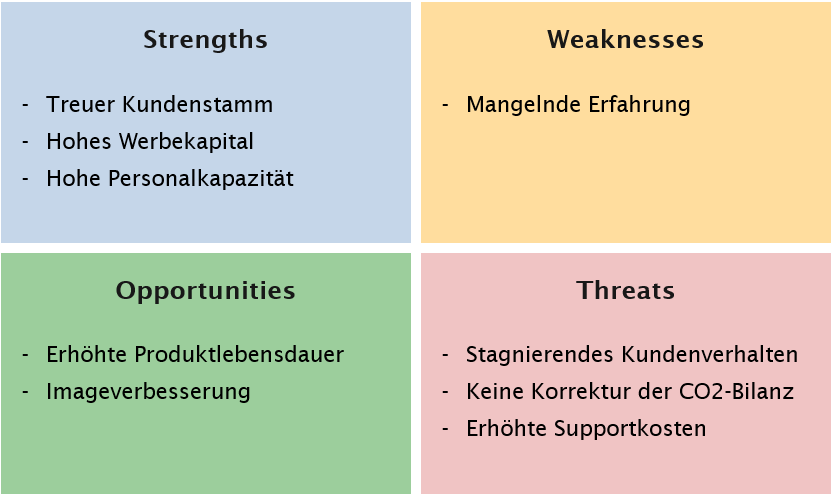
\includegraphics[width=0.9\textwidth]{SWOT}
 \caption{SWOT-Analyse zur Anwendung der neuen Designkonezpe}
 \label{fig:SWOT-Analyse}
\end{figure}


\paragraph{STÄRKEN}
\begin{itemize}
\item[•] \textbf{Treuer Kundenstamm:} 
Mit der hohen Kundezufriedenheit von 75\% bei Geschäfts- kunden und 81\% bei Privatkunden, so wie der stetig wachsenden Nachfrage nach Geräten der Marke Regularsoft und dem Vertrauen der Kunden, ist das Unternehmen bereit die Umstellung auf langlebiger Software und Modularität im Design zu nehmen.
\item[•] \textbf{Hohes Werbekapital:} 
Durch das zugewiesene Kapital  von 14,6 Mio. GE steht der Marketingabteilung des Unternehmens ausreichend finanzielle Mittel zur Verfügung, um die Produkte mit umweltfreundlicherem Design und Software stark zu vermarkten, um auch die Kunden auf die Neuerungen anzuziehen.
\item[•] \textbf{Ausreichend Personal:}
Auch an Personal fehlt es dem Unternehmen nicht. Sowohl für eine schnelle Entwicklung, als auch Vertrieb der nächsten Produktreihe stehen mit den global 600 neuen Entwicklungsmitarbeitern und 80 neuen Vertrieblern genügend Fachkräfte bereit.
\end{itemize}

\paragraph{SCHWÄCHEN}
\begin{itemize}
\item[•] \textbf{Mangelnde Erfahrung:}
Für beide Designkonzepte der Regularsoft ausreichend Erfahrung für eine schnelle Entwicklungszeit. Da bisher jegliche Software der Regularsoft mit dem traditionellen monolithischen Ansatz entwickelt wurde, konnte bis jetzt kein Know-how im Bereich der Entwicklung von modularer Software z.B. durch Microservices gesammelt werden. Ebenso sind viele technischer mit modularen Produktkonzepten noch unerfahren. Der Aufbau des erforderlichen Wissens und die Umsetzung der entsprechenden Konzepte erfordern immense Einarbeitungszeiten bei allen beteiligten Mitarbeitern.
\end{itemize}


\paragraph{CHANCEN}
\begin{itemize}
\item[•] \textbf{Erhöhte Produktlebensdauer:}
Mit den Varianten der modularen Hardwareaufbaus, als auch der Software zur Unterstützung der Hardwarekomponenten lässt sich die Lebensdauer eines einzelnen Geräts deutlich erhöhen. Während austauschbare Hardwareupgrades die Nachfrage der Kunden beibehalten und auch defekte Einheiten austauschen lässt, erreicht die langlebigerer Software, dass zwischen den Lebensdauern von Hard- und Software ein gesundes Gleichgewicht herrscht.

\item[•] \textbf{Imageverbesserung:}
Mit langlebigerer Software und Modularität als Basis der Produkte, kann Regularsoft aufgrund der gesteigerten Langlebigkeit der Produkte, dem zugänglicheren Recycling der Grundmaterialien und der insgesamt geringen Umweltbelastung, sein Firmenimage verbessern und sich umweltfreundliches und hochtechnologische Unternehmen auf den Markt positionieren. Mit Verbesserung des  grünen Images, werden auch alternative Kundengruppen die Produkte von Regularsoft in Betracht ziehen.
\end{itemize}

\paragraph{RISIKEN}
\begin{itemize}
\item[•] \textbf{Stagnierende Nachfrage:}
Damit die Umstellung umweltfreundliche Produkte erfolgreich ist, müssen vor allem die Kunden auf die Neuerungen anspringen. Kundengruppen, die jährlich neue Geräte anschaffen, könnte das Upgrade-Konzept abschrecken oder gar nicht interessieren. Währenddessen werden viele Nutzer davor zurückschrecken selbst Änderungen an Hardware vorzunehmen. Jedoch kann dies durch Upgrade-Angebote durch örtliche Filialen ausgeglichen werden. Trotzdem müssen die Kunden von Regularsoft ihr Kaufverhalten anpassen. Dieser Wandel wird längere Zeit benötigen und möglicherweise anfangs eine stagnierende Nachfrage mit sich ziehen.
\item[•] \textbf{Keine Korrektur der CO2-Bilanz:}
 Eine stagnierende Nachfrage kann jedoch auch auf die Umweltbelastung Auswirkungen haben. Zwar ermöglicht das neue Produktdesign einfacheres und besseres Recycling der verbauten Rohstoffe, jedoch kann auch eine optimales Recyclingkonzept nur zwischen 10-20\% CO2 der ursprünglichen Produktionsausstöße reduzieren. Die Umweltbelastung wird daher nur erhöht, wenn Kunden die gesteigerte Produktlebensdauer voll ausnutzen.
\item[•] \textbf{Erhöhte Supportkosten:}
Durch die längere Unterstützung von Software und deren älteren Versionen auf immer älteren Geräten fallen im Vergleich zur aktuellen Situation erheblich höhere Supportkosten an. Da zum aktuellen Zeitpunkt nicht abgeschätzt werden kann, wie sich die langlebigere Software auf das Verhalten der Kunden auswirken wird, ist es folglich nicht möglich abzuschätzen, wie lange der Support für die jeweiligen Versionen der Betriebssysteme garantiert werden muss. Dies kann in im ungünstigen Fall zu unerwartet hohen Supportkosten führen.
\end{itemize}


\end{document}
